\newcommand{\sem}[1]{\mathsf{#1}}
\newcommand{\sempred}[1]{\mathrm{#1}}

\section{Deep and shallow semantic construction}
\label{sec:motivation}

We start with an informal discussion to 
illustrate how \rmrs\ can be used to represent partial
semantic information, and why people find it useful for this purpose.
Consider the following (toy) sentence:
\begin{examples}
  \item Every fat cat chased some dog.
\end{examples}

This sentence exhibits several kinds of ambiguity, including a scope
ambiguity between ``every fat cat'' and ``some dog'' and lexical
ambiguities of the nouns ``cat'' and ``dog'' (which have 8 and 7 
WordNet senses respectively).  Simplifying slightly by
ignoring tense information (but see
Section~\ref{sec:extensions}), two of these readings are
shown as logical forms below; they can be represented as trees as
shown in Fig.~\ref{fig:1}.  

\begin{examples}
\item $\sem{\_every\_q\_1}(x, \sem{\_fat\_j\_1}(e',x) \wedge
    \sem{\_cat\_n\_1}(x),$\\
\hspace*{0.1in} $\sem{\_some\_q\_1}(y, \sem{\_dog\_n\_1}(y),$\\
\hspace*{0.2in}$\sem{\_chase\_v\_1}(e,x,y)))$
\label{ex:fat-cat-1}
\item $\sem{\_some\_q\_1}(y, \sem{\_dog\_n\_2}(y),$\\
\hspace*{0.1in}$\sem{\_every\_q\_1}(x, \sem{\_fat\_j\_1}(e',x) \wedge
    \sem{\_cat\_n\_2}(x), $\\
\hspace*{0.2in}$\sem{\_chase\_v\_1}(e,x,y)))$
\label{ex:fat-cat-2}
\end{examples}


\begin{figure*}[t]
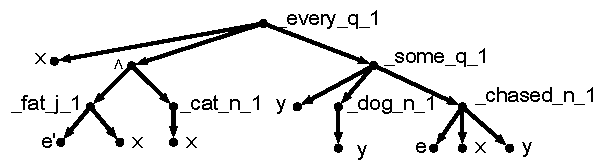
\includegraphics[width=6cm]{pic-cat-chased-dog}
\hspace{1cm}
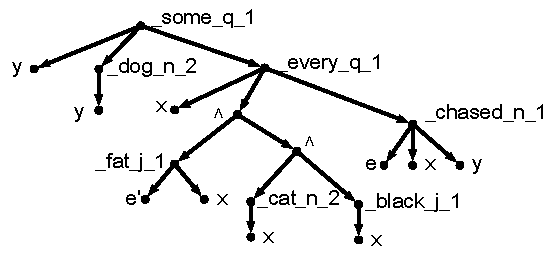
\includegraphics[width=6cm]{pic-cat-chased-dog-2}
\caption{Structure trees of the semantic representations (\ref{ex:fat-cat-1}) and
  (\ref{ex:fat-cat-2}). \label{fig:1}}
\end{figure*}


Now imagine trying to extract semantic information from
the output of a part-of-speech tagger by using the word lemmas as
lexical predicate symbols.  Such a semantic representation is highly
partial, as it will not say anything about predicate-argument
relations or resolve lexical ambiguity---it will use predicate
symbols such as $\sempred{\_cat\_n}$, which might resolve to the
predicate symbols $\sem{\_cat\_n\_1}$ or $\sem{\_cat\_n\_2}$ in the
complete semantic representation.  (Notice the different
fonts for the ambiguous and unambiguous predicate symbols.)  
We can
express this information in \rmrs\ as follows.

\begin{examples}
\item \label{ex:cat-pos}
$l_1:a_1:\sempred{\_every\_q}(x_1)$, \\
$l_{41}:a_{41}:\sempred{\_fat\_j}(e')$,\\
$l_{42}:a_{42}:\sempred{\_cat\_n}(x_3)$\\
$l_5:a_5:\sempred{\_chase\_v}(e)$, \\
$l_6:a_6:\sempred{\_some\_q}(x_6)$, \\
$l_9:a_9:\sempred{\_dog\_n}(x_7)$
\end{examples}

This \rmrs\ consists of six \emph{elementary predications} ({\sc ep}s), one
for each word lemma in the sentence; each of them is prefixed by a
\emph{label} and an \emph{anchor}, which are essentially variables
that refer to nodes in the trees in Fig.~\ref{fig:1}.  
The lack of semantic dependencies rendered by a {\sc pos} tagger
means we have unique arguments to each
predicate symbol (e.g., see $x_1$ and $x_3$ in (\ref{ex:cat-pos}),
compared with the {\em same} variable $x$ in the semantic
representations (\ref{ex:fat-cat-1}) and (\ref{ex:fat-cat-2})).
We can say that
the two trees \emph{satisfy} this \rmrs\ because it is possible to map
the labels and anchors into nodes in each tree and variable names like
$x_1$ and $x_3$ into variable names in the tree in such a way that the
predication
of
the node that labels and anchors are mapped to is consistent with
that given in the {\sc ep}s of the {\sc rmrs}.
For instance, the first tree satisfies
the \rmrs\ because $l_1$ and $a_1$ can map to the root of that
tree and $x_1$ to $x$, and the root label
$\sem{\_every\_q\_1}$ is consistent with the 
{\sc ep} predicate $\sempred{\_every\_q}$.

There are of course many other trees (and thus, fully specific
semantic representations such as (\ref{ex:fat-cat-1})) that are
described equally well by the \rmrs\ (\ref{ex:cat-pos}); this is
not surprising, 
given that the semantic information we got from the {\sc pos} tagger is so
incomplete.  If we have more information, say information about
subject and object relations from a chunk parser like Cass
\cite{abney:1996}, we can represent these in a more
detailed \rmrs, as follows:

\begin{examples}
\item 
$l_1:a_1:\sempred{\_every\_q}(x_1)$, \\
$l_{41}:a_{41}:\sempred{\_fat\_j}(e')$,\\
$l_{42}:a_{42}:\sempred{\_cat\_n}(x_3)$\\
$l_5:a_5:\sempred{\_chase\_v}(e)$, \\
\hspace*{0.1in} $\ARG1(a_5,x_4),
\ARG2(a_5,x_5)$\\ 
$l_6:a_6:\sempred{\_some\_q}(x_6)$, \\
$l_9:a_9:\sempred{\_dog\_n}(x_7)$\\
$x_3=x_4$, $x_5=x_7$
\label{ex:cat-partial-parser}
\end{examples}

This \rmrs\ uses two new types of atoms.  Atoms of the form $x_3=x_4$
express that the two variables $x_3$ and $x_4$ must map to the same
variable in any fully specific logical form; e.g., to the variable $x$
in Fig.~\ref{fig:1}.  Atoms of the form
$\ARG_i(a,z)$ and $\ARG_i(a,h)$ express that the $i$-th child
(counting from 0) of the
node to which the anchor $a$ refers is the variable name that $z$ denotes
(or the node that the {\em hole} $h$ denotes).  The separation of
{\sc ep}s and $\ARG$ atoms is perhaps the most important difference between
\rmrs\ and earlier underspecification formalisms such as \mrs\ and
dominance graphs, which required that a predicate and its arguments
had to be specified together.  \rmrs\ goes beyond these formalisms in
expressive power, because it allows one to state separately
information about how many arguments a predicate takes (which is
necessary for supporting parsers where information about lexical
subcategorisation is absent), and the values of
those (non-scopal and scopal) arguments.   If we also allow atoms of the form
$\ARG_{\{2,3\}}(a,x)$ to express uncertainty as to whether $x$ is the
second or third child of the anchor $a$, then \rmrs\ can specify the
arguments to a predicate while underspecifying their position. 

Finally, \rmrs\ (\ref{ex:cat-erg}) is a notational variant of the {\sc
  mrs} derived by the {\sc erg}, a wide-coverage deep grammar:
\begin{examples}
\item $l_1:a_1\handel\mbox{\_every\_q\_1}(x_1),$\\
\hspace*{0.1in}$\mbox{RSTR}(a_1,h_2),
\mbox{BODY}(a_1,h_3)$\\ 
$l_{41}:a_{41}\handel\mbox{\_fat\_j\_1}(e'), \ARG1(a_{41},x_2)$\\
$l_{42}:a_{42}\handel\mbox{\_cat\_n\_1}(x_3)$\\
$l_5:a_5\handel\mbox{\_chase\_v\_1}(e)$,\\
\hspace*{0.1in}$\ARG1(a_5,x_4),
\ARG2(a_5,x_5)$\\ 
$l_6:a_6\handel\mbox{\_some\_q\_1}(x_6)$,\\
\hspace*{0.1in}$\mbox{RSTR}(a_6,h_7),
\mbox{BODY}(a_6,h_8)$\\ 
$l_9:a_9\handel\mbox{\_dog\_n\_1}(x_7)$\\
$h_2=_q l_{42}, l_{41}=l_{42}, h_7 =_q l_9$\\
$x_1=x_2, x_2=x_3, x_3=x_4,$\\
$x_5=x_6, x_5=x_7$
\label{ex:cat-erg}
\end{examples}
RSTR and BODY are conventional names for the scopal arguments to
predicate symbols corresponding to quantifiers.   
Atoms like $h_2 \qeq l_{42}$ specify
a kind of ``outscopes'' relationship between the hole and the label,
and can be used to underspecify the scope of the two quantifiers.
Notice also that the labels of the {\sc ep}s for ``fat'' and ``cat'' are
stipulated to be equal in the \rmrs\ (\ref{ex:cat-erg}), whereas the
anchors are not. 
In the tree, it is the anchors that are mapped to the nodes with the
labels $\sem{\_fat\_j\_1}$ and $\sem{\_cat\_n\_1}$; the label is
mapped to the conjunction node just above them.  In other words, the
role of the anchor in an {\sc ep} is to connect a predicate to its
arguments, while the role of the label is to connect the {\sc ep} to the
surrounding formula.  Representing conjunction with label sharing
stems from \mrs\ and provides compact semantic representations.
Finally, (\ref{ex:cat-erg}) intuitively represents more specific
semantic information than (\ref{ex:cat-pos}), so long as
the constructors that \_cat\_n\_1 can correspond to is a
subset of those that \_cat\_n can correspond to (written
$\mbox{\_cat\_n\_1}\sqsubseteq \mbox{\_cat\_n}$), and similarly for
\_fat\_j\_1 etc.  This is because with these so-called SPEC relations
on the predicate symbols in place, (\ref{ex:cat-erg}) simply adds
ARGs, qeqs and variable equalities to (\ref{ex:cat-pos}).

In summary, \rmrs\ is a formalism for representing partial information
about semantic representations.  It can
represent the output of a deep grammar in a way that is a notational
variant of \mrs; but in cases in which a deep grammar is not
available, it can be used to capture whatever partial semantic
information a shallower {\sc nlp} tool can provide.  \rmrs\ is
designed to be a generic formalism for partial semantic
representations which abstracts over the details of different {\sc nlp}
tools and allows us to represent, process, and compare information
from different tools in the same formalism, and in the long run
provide a platform for incrementally enriching partial information
such as (\ref{ex:cat-pos}) in order to eventually approximate more
detailed representations such as (\ref{ex:cat-partial-parser}) or
(\ref{ex:cat-erg}).

However, although people have started using \rmrs\ in their
implemented systems, it is still relatively ad-hoc in that its formal
syntax is not consistent across different papers, and its formal
semantics is not defined; we don't know, formally, what an \rmrs\
\emph{means} in terms of semantic representations like
(\ref{ex:fat-cat-1}) and (\ref{ex:fat-cat-2}), and this hinders our
ability to design efficient algorithms for processing \rmrs. The
purpose of this paper is to lay the groundwork for fixing this problem.

%%% Local Variables: 
%%% mode: latex
%%% TeX-master: "rmrs-08"
%%% End: 
